\subsection{Separated maps}

PROPOSITION 1. --- Let X and Y be topological spaces, and let \(f\colon X \to Y\) be a continuous map. The following properties are equivalent:

\begin{enumerate}
\def\labelenumi{(\roman{enumi})}
\item
  The diagonal \(\Delta_{X}\) of the fibered product X \(\times_{Y}\) X is a closed subspace;
\item
  For every topological space W and every pair of continuous maps \((g_{1}, g_{2})\) from W into X such that \(f \circ g_{1} = f \circ g_{2}\) , the set of points \(w \in W\) such that \(g_{1}(w) = g_{2}(w)\) is closed in W;
\item
  For every pair \((x_{1}, x_{2})\) of points of X such that \(x_{1} \neq x_{2}\) and \(f(x_{1}) = f(x_{2})\) , there exists a neighborhood \(V_{1}\) of \(x_{1}\) in X and a neighborhood \(V_{2}\) of \(x_{2}\) in X such that \(V_{1} \cap V_{2} = \varnothing\) .
\end{enumerate}

(i)⇒(ii): Let \(g_{1}\) and \(g_{2}\) be continuous maps from W into X such that \(f \circ g_{1} = f \circ g_{2}\), and let \(g: W \to X \times_{Y} X\) be the map induced by \(g_{1}\) and \(g_{2}\). The set of points \(w \in W\) such that \(g_{1}(w) = g_{2}(w)\) is \(g^{-1}(\Delta_{X})\). Since g is continuous, it is therefore closed if the diagonal \(\Delta_{X}\) is closed.

(ii)⇒(i): The diagonal \(\Delta_{X}\) is the set of points \(z \in X \times_{Y} X\) such that \(\mathrm{pr}_{1}(z) = \mathrm{pr}_{2}(z)\). It follows from (ii), applied to \(W = X \times_{Y} X\) and to the pair of maps \((\mathrm{pr}_{1}, \mathrm{pr}_{2})\), that the diagonal \(\Delta_{X}\) is closed in \(X \times_{Y} X\).

(i)⇔(iii): Let \((x_{1}, x_{2})\) be a point of \(X \times_{Y} X\) and let \(V_{1}\) and \(V_{2}\) be neighborhoods of \(x_{1}\) and \(x_{2}\), respectively. The condition \(V_{1} \cap V_{2} = \varnothing\) is equivalent to the condition \((\mathrm{V}_{1} \times \mathrm{V}_{2}) \cap \Delta_{\mathrm{X}} = \varnothing\), that is, to \((\mathrm{V}_{1} \times \mathrm{V}_{2}) \cap (\mathrm{X} \times_{\mathrm{Y}} \mathrm{X}) \cap \Delta_{\mathrm{X}} = \varnothing\). Since the sets \((\mathrm{V}_{1} \times \mathrm{V}_{2}) \cap (\mathrm{X} \times_{\mathrm{Y}} \mathrm{X})\) form a base of neighborhoods of \((x_{1}, x_{2})\) in \(X \times_{Y} X\), this proves the equivalence of (i) and (iii).

DEFINITION 1. --- Let X and Y be topological spaces. A continuous map \(f: X \to Y\) is separated if it satisfies the equivalent conditions of Proposition 1.

PROPOSITION 2. --- Let X, Y, Z be topological spaces and let \(f\colon X \to Y\) and \(g\colon Y \to Z\) be continuous maps.

\begin{enumerate}
\def\labelenumi{\alph{enumi})}
\item
  If f and g are separated, then \(g \circ f\) is separated.
\item
If g \(\circ\) f is separated, then f is separated.
\item
  Suppose further that the map f is proper and surjective. Then, if g ∘ f is separated, g is separated.
\end{enumerate}

Consider, in X×X, the subspaces \(\Delta_{X}\) (diagonal), \(X \times_Y X\) and \(X \times_Z X\). These are respectively the sets of points u of X×X such that \(\mathrm{pr}_{1}(u)=\mathrm{pr}_{2}(u)\), \(f\circ\mathrm{pr}_{1}(u)=f\circ\mathrm{pr}_{2}(u)\), \(g\circ f\circ\mathrm{pr}_{1}(u)=g\circ f\circ\mathrm{pr}_{2}(u)\). If \(g\circ f\) is separated, \(\Delta_{X}\) is closed in \(X \times_Z X\), hence also in \(X \times_Y X\), whence b).

By Proposition 1, (ii), applied to W = X ×\_Z X, \(g_1 = f \circ \text{pr}_1\) and \(g_2 = f \circ \text{pr}_2\), X ×\_Y X is closed in X ×\_Z X if \(g\) is separated. If moreover \(f\) is separated, \(\Delta_X\) is closed in X ×\_Y X (Proposition 1, (i)), hence in X ×\_Z X, whence \(a\).

Finally, let us prove \(c\). The map \((f, f) \colon X \times X \to Y \times Y\) is proper (TG, I, p. 73, prop. 4). The subspace \(X \times_Z X\) is the inverse image of \(Y \times_Z Y\) under \((f, f)\); by TG, I, p. 72, prop. 3, the map \(u \colon X \times_Z X \to Y \times_Z Y\) induced by \((f, f)\) is proper. Since \(g \circ f\) is separated, the diagonal \(\Delta_X\) is closed in \(X \times_Z X\). Consequently, \(u(\Delta_X)\) is closed in \(Y \times_Z Y\). Since \(f\) is surjective, \(u(\Delta_X)\) is the diagonal of \(Y \times_Z Y\). This shows that \(g\) is separated.

Remarks. --- 1) An injective continuous map is separated.

\begin{enumerate}
\def\labelenumi{\arabic{enumi})}
\setcounter{enumi}{1}
\tightlist
\item
  For a topological space X to be Hausdorff (TG, I, p. 52, def. 1), it is necessary and sufficient that the map from X into a space reduced to a single point be separated. In this case, every continuous map from X into a topological space is separated (Proposition 1, (iii)).
\end{enumerate}

Let \(f\colon X \to Y\) be a continuous and separated map. For every point \(y\) of \(Y\), the fiber \(f^{-1}(y)\) is a separated topological space (loc. cit.). There nevertheless exist continuous maps which are not separated but all of whose fibers are separated topological spaces (I, p. 140, exerc. 1).

\begin{enumerate}
\def\labelenumi{\arabic{enumi})}
\setcounter{enumi}{2}
\item
  Let \(f \colon X \to Y\) be a continuous and separated map. If the space Y is separated, then the space X is separated. This follows from Remark 2 and Proposition 2 applied with a space Z reduced to a point.
\item
  Let \(f \colon X \to Y\) be a continuous and separated map, let \(y\) be a point of \(Y\), and let \(A\) be a finite subset of \(f^{-1}(y)\). Let us prove that there exists a family \((V_a)_{a \in A}\) of pairwise disjoint sets such that, for each \(a \in A\), the set \(V_a\) is a neighborhood of \(a\) in X. To do this, for each subset \(\{a,b\}\) of \(A\) with two elements, choose a neighborhood \(V_{(a,b)}\) of \(a\) and a neighborhood \(\mathrm{V}_{(b,a)}\) of \(b\) in X such that \(\mathrm{V}_{(a,b)} \cap \mathrm{V}_{(b,a)} = \varnothing\) (Proposition 1, (iii)). Let \(\mathrm{V}_a\) denote the intersection of the family formed by X and the sets \(\mathrm{V}_{(a,b)}\) for \(b \in \mathrm{A}\), \(b \neq a\). The set \(\mathrm{V}_a\) is a neighborhood of \(a\) in X, and if \(a\), \(b\) are two distinct elements of A, the set \(\mathrm{V}_a \cap \mathrm{V}_b\) is contained in \(\mathrm{V}_{(a,b)} \cap \mathrm{V}_{(b,a)}\), hence is empty.
\item
  Let \(Y\) be a topological space. Let \((\mathrm{A}_{i})_{i\in\mathrm{I}}\) be a family of subsets of Y and let X be the sum space of the family \((\mathrm{A}_{i})_{i\in\mathrm{I}}\). The canonical map from X to Y is separated.
\end{enumerate}

PROPOSITION 3. --- Let \(f\colon X \to Y\) be a continuous and separated map. Every continuous section of \(f\) induces a homeomorphism of \(Y\) onto a closed subset of \(X\).

Let \(s\colon Y \to X\) be a continuous section of \(f\). The map \(s\) induces a homeomorphism of \(Y\) onto the subspace \(s(Y)\) of \(X\) (TG, I, p. 22, prop. 9). The identity map of \(X\) and the map \(s \circ f\) are continuous and one has \(f \circ \mathrm {Id}_{X} = f \circ (s \circ f)\). Since the map \(f\) is separated, the set \(s(Y)\), which is the set of points \(x\) of \(X\) such that \(x = (s \circ f)(x)\), is closed in \(X\) (Proposition 1, (ii)).

PROPOSITION 4. --- Let

\pandocbounded{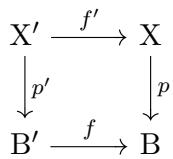
\includegraphics[keepaspectratio]{images/part001_94ec13ba.jpg}}

a Cartesian square. If the map p is separated, then so is p'. Conversely, if p' is separated and if f is universally strict and surjective, then p is separated.

Consider the square

\[
\begin{array}{c} \mathrm {X^ {\prime} \times_ {B^ {\prime}} X^ {\prime}} \xrightarrow {\varphi} \mathrm {X \times_ {B} X} \\ \Biggl \downarrow_ {q ^ {\prime}} \\ \mathrm {B^ {\prime} \xrightarrow {f} B} \end{array}
\]

where the map \(\varphi\) is induced by the map \(f' \times f': X' \times X' \to X \times X\) . Recall (I, p. 13, example 1) that this square is Cartesian and that one has \(\overline{\varphi}^1(\Delta_X) = \Delta_{X'}\) .

If the map p is separated, the set \(\Delta_{\mathrm{X}}\) is closed in \(\mathrm{X} \times_{\mathrm{B}} \mathrm{X}\); therefore, \(\Delta_{\mathrm{X}'}\) is a closed subset of \(\mathrm{X}' \times_{\mathrm{B}'} \mathrm{X}'\), which proves that the map \(p'\) is separated.

If the map f is surjective, the map \(\varphi\) is surjective (I, p. 10, cor.); if f is universally strict, \(\varphi\) is strict (I, p. 20, def. 6). Suppose the map \(p'\) is separated. Then \(\Delta_{\mathrm{X}'}\) is closed in \(\mathrm{X}' \times_{\mathrm{B}'} \mathrm{X}'\). Since \(\Delta_{\mathrm{X}'} = \overline{\varphi}^{1}(\Delta_{\mathrm{X}})\) and since \(\varphi\) is surjective and strict, \(\Delta_{\mathrm{X}}\) is closed in \(\mathrm{X} \times_{\mathrm{B}} \mathrm{X}\), which proves that the map \(p\) is separated.

PROPOSITION 5. --- Let \(f: X \to Y\) and \(g: Y \to Z\) be continuous maps. Suppose the map \(g\) is separated and the map \(g \circ f\) is proper. The map \(f\) is then proper.

Consider the following Cartesian square:

\[
\begin{array}{c} \mathrm{X} \times_ {\mathrm{Z}} \mathrm{Y} \xrightarrow {\operatorname{pr} _ {2}} \mathrm{Y} \\ \Biggl \downarrow \operatorname{pr} _ {1} \\ \mathrm{X} \xrightarrow {g \circ f} \mathrm{Z}. \end{array}
\]

Let \(s \colon X \to X \times_{Z} Y\) be the map \(x \mapsto (x, f(x))\). This is a continuous section of \(\mathrm{pr}_1 \colon X \times_{Z} Y \to X\). By Proposition 4, the map \(\mathrm{pr}_1\) is separated; it follows that the map \(s\) is proper (I, p. 27, prop. 3 and TG, I, p. 72, prop. 2). On the other hand, the map \(\mathrm{pr}_2\) is proper (I, p. 17, prop. 8). Therefore the map \(f\), which is equal to \(\mathrm{pr}_2 \circ s\), is proper (TG, I, p. 73, prop. 5).

